\documentclass[a4paper]{scrreprt}

%%% PACKAGES %%%

% add unicode support and use german as language
\usepackage[utf8]{inputenc}
\usepackage[ngerman]{babel}
% Use Helvetica as font
\usepackage[scaled]{helvet}
\renewcommand\familydefault{\sfdefault}
\usepackage[T1]{fontenc}
% Better tables
\usepackage{tabularx}
% Better enumerisation env
\usepackage{enumitem}
% Use graphics
\usepackage{graphicx}

%%% COMMAND REBINDINGS %%%
\newcommand{\tabitem}{~~\llap{\textbullet}~~}

%%% PATH DEFINITIONS %%%
% Define the path were images are found
\graphicspath{{./img/}{./pdf/}}

%%% TITLEPAGE %%%

\title{Projektdokumentation}
\subtitle{PAWI HS18}
\author{Pascal Baumann, Dane Wicki}
\date{\today}

\begin{document}

\begin{titlepage}
\maketitle
\end{titlepage}

\section*{Versionskontrolle}

\begin{tabularx}{\textwidth}{|c|c|c|X|}
	\hline 
	\textbf{Versionsnummer} & \textbf{Kürzel} & \textbf{Datum} & \textbf{Beschreibung} \\ 
	\hline 
	0.1 & PB & 10.09.18 & Erste Versionierung \\ 
	\hline 
\end{tabularx} 

\tableofcontents

\chapter{Systemspezifikation}

\section{Systemübersicht}

\section{Architektur \& Design}

\section{Schnittstellen}

\section{Anforderungen}

\section{Anwendung}

\chapter{Projektmanagementplan}

\section{Projektorganisation}
Da beide Projektmitglieder ihre Kompetenzen eher in den technischen Bereichen dieses Projekts sehen, wurde von einer strikten Aufgabenteilung abgesehen.

Es wurde dennoch darauf geachtet, dass beide Mitglieder klare Verantwortungen übernehmen. Diese waren jedoch mehr in einer überwachenden Funktion gesehen, und soll nicht heissen, dass dieses Mitglied die Arbeit alleine leistete.

\vspace{1em}

\begin{tabularx}{\textwidth}{|X|X|}
	\hline
	\textbf{Teammitglied} & \textbf{Funktionen} \\
	\hline
	Pascal Baumann & \tabitem Dokumentation \\
	& \tabitem Testplanung \& Durchführung \\
	& \tabitem Projektmanagement \\
	\hline
	Dane Wicki & \tabitem Architektur \\
	& \tabitem Plattformanalyse \\
	\hline
\end{tabularx}

\section{Projektführung}

\subsection{Rahmenplan}

Das Projekt wurde in 7 zweiwöchige Sprints unterteilt und in diesen iterativ entwickelt.

\vspace{1em}

\begin{figure}
	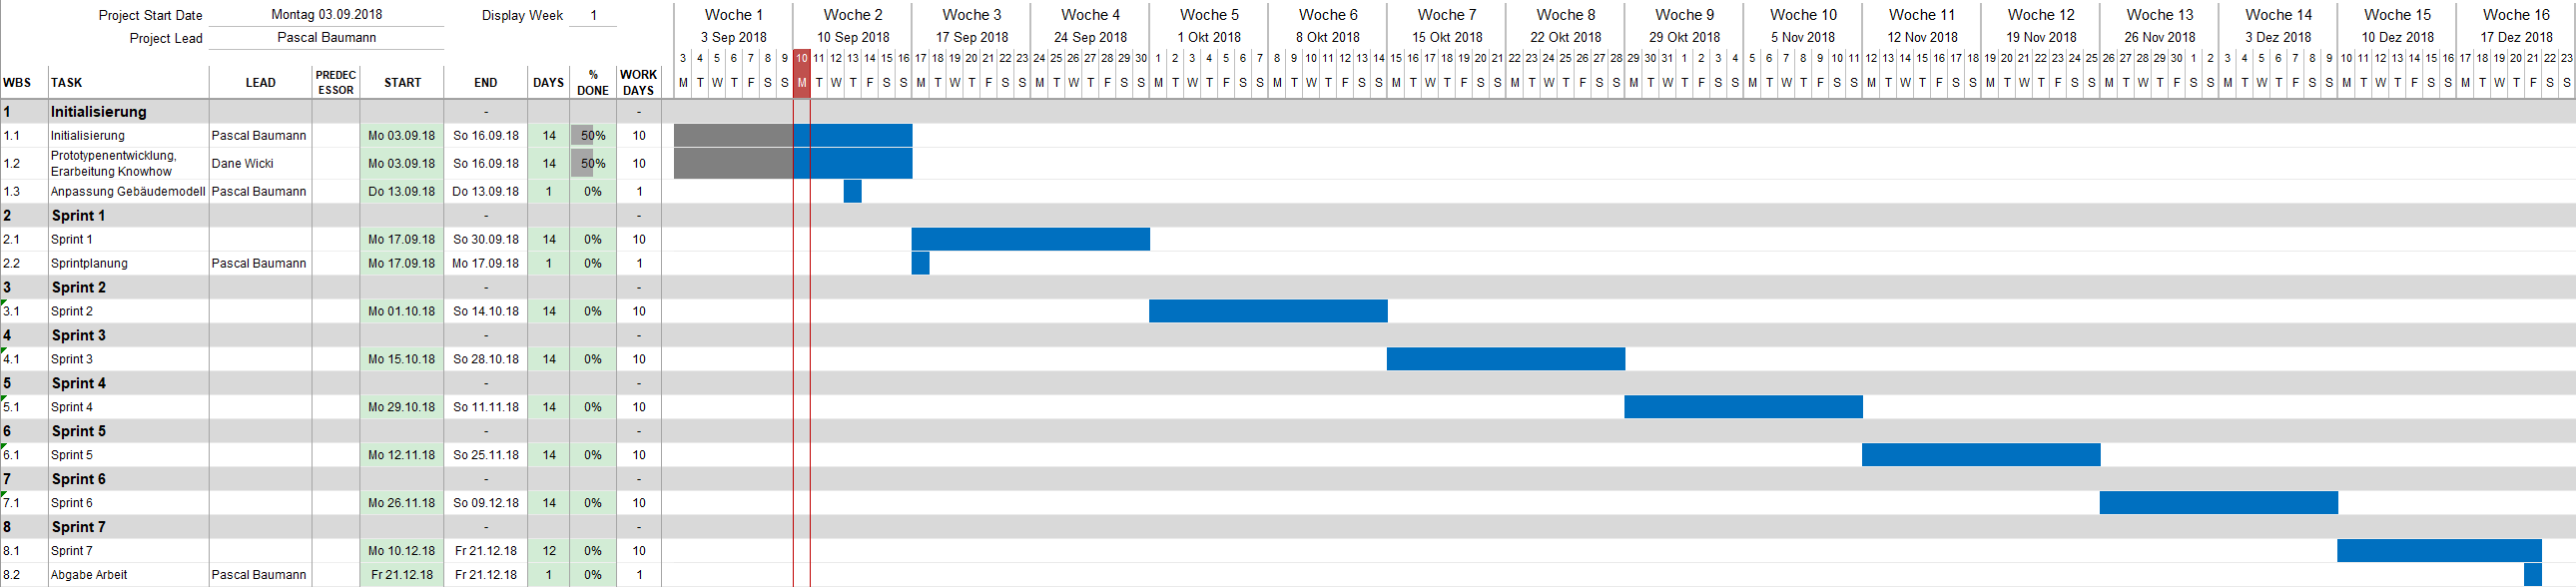
\includegraphics[keepaspectratio, width=\textwidth]{Rahmenplan}
	\caption{Überblick der Sprints}
\end{figure}

\section{Projektabwicklung}

\section{Testplan}

\section{Testfälle}

\section{Testprotokolle}

\bibliography{Referenzen.bib}
\appendix

\end{document}